\documentclass[11pt,letterpaper]{article}

% Math stuff
\usepackage{amsmath, amsfonts, mathtools, amsthm, amssymb}
% Fancy script capitals
\usepackage{mathrsfs}
\usepackage{cancel}
% Bold math
\usepackage{bm}
\usepackage{pgfplots}
\pgfplotsset{compat=1.17}
\usepackage{tikz}
\usepackage{quiver}
% Geometry
\usepackage[letterpaper, portrait, margin=1.25in, includefoot]{geometry}


\providecommand{\bE}{\mathbf{E}}
\providecommand{\bB}{\mathbf{B}}
\providecommand{\bJ}{\mathbf{J}}
\providecommand{\bj}{\mathbf{j}}
\providecommand{\bff}{\mathbf{f}}
\providecommand{\VF}{\mathfrak{X}}

\providecommand{\R}{\mathbb{R}}
\providecommand{\C}{\mathbb{C}}
\providecommand{\Z}{\mathbb{Z}}
\providecommand{\RP}{\mathbb{RP}}
\providecommand{\Hom}{\mathrm{Hom}}
\providecommand{\CC}{\mathscr{C}}
\providecommand{\Eq}{\mathrm{Eq}}
\providecommand{\Coeq}{\mathrm{Coeq}}
\providecommand{\hCW}{\mathbf{hCW}}
\providecommand{\Set}{\mathbf{Set}}
\providecommand{\colim}{\mathrm{colim}}
\providecommand{\Th}{\mathrm{Th}}

\newcommand\defn[1]{\textbf{#1}}
\newcommand\todo[1]{{\color{red}\textbf{#1}}}

\theoremstyle{definition}
\newtheorem{definition}{Definition}[subsection]
\newtheorem{theorem}[definition]{Theorem}
\newtheorem{remark}[definition]{Remark}
\newtheorem{proposition}[definition]{Proposition}
\newtheorem{claim}[definition]{Claim}
\newtheorem{lemma}[definition]{Lemma}
\newtheorem{example}[definition]{Example}
\newtheorem{corollary}[definition]{Corollary}

% Restriction
\newcommand\restr[2]{{
  \left.\kern-\nulldelimiterspace
  #1
  \vphantom{\big|}
  \right|_{#2}
}}

\edef\restoreparindent{\parindent=\the\parindent\relax}
\usepackage{parskip}
\restoreparindent

\usepackage[shortlabels]{enumitem}
\setlist[enumerate]{topsep=1ex,itemsep=1ex,partopsep=1ex,parsep=1ex}
\setlist[itemize]{topsep=1ex,itemsep=1ex,partopsep=1ex,parsep=1ex}

\renewcommand{\abstractname}{Summary}    % clear the title


\title{\textbf{Math 55a Problem Set 10}}

\begin{document}
\maketitle
\setcounter{page}{0}
\thispagestyle{empty}

\begin{itemize}
  \item How long did this assignment take you? -- 10 hours
  \item How hard was it? -- Tough
  \item What resources did you use and how much help did you need? -- Collaborated with AJ LaMotta
  \item Did you have any prior experience with this material? -- No
\end{itemize}

\pagebreak
\begin{problem}
Let $p$ and $q$ be distinct primes. Show that a group of order $pq$ or $p^2q$ cannot be simple.
\end{problem}
Let $s_p$ be the number of Sylow $p$-subgroups of $G$.

\textbf{Case $|G|=pq$:} Here $s_p=1$ or $q$ and $s_q=1$ or $p$. If either $s_p$ or $s_q$ is equal to one then we are done, since this gives a normal subgroup of $G$ by the second Sylow theorem. So suppose for the sake of contradiction that $s_p=q$ and $s_q=p$. Then by the third Sylow theorem, $p\equiv 1\mod q$ and $q\equiv 1\mod p$. This is impossible because if $p=1+qn$ and $q=1+pm$ then $p=1+(1+pm)n$ so $(mn-1)p=-1-n$. 

\textbf{Case $|G|=p^2q$:} Here $s_p=1$ or $q$ and $s_q=1, p$, or $p^2$. As before, if either $s_p$ or $s_q$ are equal to one then we are done. So suppose $s_p=q$ and $s_q=p$ or $p^2$. Here $q\equiv 1\mod p$ and $s_q\equiv 1\mod q$. In both cases, a similar argument gives a numeric contradiction, proving that the group must always be simple.

\pagebreak
\begin{problem}
How many groups of order 33 are there, up to isomorphism?
\end{problem}
Let $s_p$ be the number of Sylow $p$-subgroups of $G$. We claim that such a group must have a single Sylow 3-subgroup and a single Sylow 11-subgroup. This is because $s_3|11$ and $s_3\equiv 1\mod 3$ so $s_3=1$ and $s_{11}|3$ and $s_{11}\equiv 1\mod 3$ so $s_{11}=1$. Thus by the direct product criterion, $G=\Z/3\times \Z/11=\Z/33$ is the only group of order $33$.

\pagebreak
\begin{problem}
How many groups of order 18 are there, up to isomorphism?
\end{problem}

Let $s_p$ be the number of Sylow $p$-subgroups of $G$. First we'll show that $G$ must have a normal subgroup of order $9$. We know that $s_3\equiv 1\mod 3$ and $s_3|2$. Hence $s_3=1$. Denote this subgroup by $N$. Choosing some other subgroup $H$ of order $2$, we can decompose $G$ as $G=N\rtimes H$. Now $H$ can only be the group $\Z/2$ because this is the only group of order 2, but $N$ can be $\Z/9$ or $\Z/3\times\Z/3$, since these are the only two groups of order $9$. So we must classify the semidirect products $\Z/9\rtimes \Z/2$ and $(\Z/3\times \Z/3)\rtimes \Z/2$.

\textbf{Case $\Z/9\rtimes \Z/2$:} Any automorphism of $\Z/9$ is of the form $x\mapsto x^k$ for some $k$ with $\gcd(n,k)=1$. So our group $G$ has presentation 
\[
    \big\langle x,y \mid x^9=y^2=1, yxy=x^k \big\rangle
.\] 
Examining these relations, we get $x=y^2xy^2=x^{k^2}$. So $k^2\equiv 1\mod 9$. The only such $k$ are $k=1$ or $k=-1$. If $k=1$, then $G$ is abelian since $yx=xy$, thus the group is \mybox{$\Z/18$} since $9$ and $2$ are coprime. Alternatively, if $k=-1$, our group has the presentation
\[
    \big\langle x,y \mid x^9=y^2=1, yx=x^{-1}y \big\rangle
.\] 
This is exactly the dihedral group \mybox{$D_{18}$}.

\textbf{Case $(\Z/3\times \Z/3)\rtimes \Z/2$:} In this case, any automorphism of $\Z/3\times \Z/3$ is an element of the general linear group $\GL(2, \F_3)$. We are specifically looking for some automorphism $T\in \GL(2,\F_3)$ such that $T^2=I$, since the semidirect product $(\Z/3\times \Z/3)\rtimes \Z/2$ is determined by a homomorphism $\Z/2\to\GL(2,\F_3)$. Since $T^2-I$ decomposes into linear factors, it follows that $T$ must be diagonalizable so it has eigenvalues which are either $1$ or $-1$. There are three possible cases. If both eigenvalues are $1$, the product is direct so the group is \mybox{$\Z/6\times\Z/3$}. If one eigenvalue is $1$ and the other is $-1$, then we have a group with presentation
\[
    \big\langle x,y,z \mid x^3=y^3=z^2=1, zx=xz, zy=y^{-1}z \big\rangle = \Z/3 \times \big\langle y,z \mid y^3=z^2=1, zy=y^{-1}z\big\rangle
.\] 
Here $x,y$ can be thought of as the eigenvectors of $T$ in $\Z/3\times \Z/3$. This group is exactly \mybox{$S_3\times \Z/3$}. The last case is when both eigenvalues are $-1$, in which case we have the presentation
\[  
    \big\langle x,y,z \mid x^3=y^3=z^2=1, zx=x^{-1}z, zy=y^{-1}z \big\rangle
.\]     
This group is commonly called the {\em generalized dihedral group} and is denoted by \mybox{$\mathrm{Dih}(\Z/3\times\Z/3)$}.

So to summarize there are exactly $5$ groups of order $18$.

\pagebreak
\begin{problem}
Prove that, if $n=pq$ is a product of primes such that $p|(q-1)$, then there exists a {\em unique} non-abelian group of order $n$ up to isomorphism.
\end{problem}

Let $s_p$ be the number of Sylow $p$-subgroups of $G$. We've established in Problem~1 that if $s_p=1$ and $s_q=1$ then the group must be abelian so we don't care about this. We've also shown that it's impossible for $s_p=q$ and $s_q=p$ at the same time. So the only cases we have are when $s_p=q$ and when $s_p=1$ or when $s_p=1$ and $s_q=p$.

\textbf{Case $s_p=1$, $s_q=p$:} This is impossible because by the third Sylow theorem $p\equiv 1\mod q$ yet by assumption $q\equiv 1\mod p$. (See Problem~1 for more details)

\textbf{Case $s_p=q$, $s_q=1$:} Here we have a normal subgroup of size $q$ which must be isomorphic to $\Z/q$ so the group must be of the form $G=\Z/q\rtimes \Z/p$. Every automorphism of $\Z/q$ is of the form $x\mapsto x^k$ and by the argument in Problem~3, we must have $k^p\equiv 1\mod q$. So $k$ is some root of the polynomial $x^p-1$ in $\F_q[x]$.

Since $p|(q-1)$, the roots of this polynomial are $1$ and the elements of order $p$ in $\F_q$. These elements form a subgroup of $\F_q^\times$ or order $p$. Let's call this subgroup $H$. Since it has order $p$, it must be cyclic, and let $g\in H$ be some generator of $H$. We claim that $G$ is isomorphic to the group
\[
    G_g = \big\langle x,y \mid x^q=y^p=1, yxy^{-1}=x^{g} \big\rangle
.\] 
We know that $G$ must be isomorphic to some $G_{g^k}$ where $k\neq 0$ by the argument in the previous paragraph, so it suffices to show that $G_{g}\cong G_{g^k}$ for all $k\neq 0$. Consider the homomorphism
\[
    \Phi_k : G_g \to G_{g^k}
\]     
which sends $y \mapsto y$ and $x\mapsto x^{g^{k-1}}$. Observe that $\Phi_k(y)^p=1$,  $\Phi_k(x)^q=x^{qg^{k-1}}=1$, and $\Phi_k(y)\Phi_k(x)\Phi_k(y)^{-1}=yx^{g^{k-1}}y^{-1}=x^{g^k}$. So $\Phi_k$ maps the generators of $G_g$ to the generators of $G_{g^{k}}$ and both groups have the same size, hence $\Phi_k$ is an isomorphism. So the only non-abelian group of order $pq$ is $G_g$.

\pagebreak
\begin{problem}
The dihedral group $D_n$ of symmetries of a regular $n$-gon is generated
by a pair of reflections $s,t$ whose axes make an angle of $\pi/n$.

\begin{enumerate}[(a)]
    \item Describe the Cayley graph of $D_n$ with respect to the generators $\{s,t\}$. How are the various types of elements of $D_n$ expressed by words in terms of $s$ and $t$?
    \item Let $G$ be the quotient of the free group on two generators $\sigma,\tau$ by the smallest normal subgroup containing $\sigma^2$ and $\tau^2$. Describe all elements of $G$, by giving a list of words in the generators $\sigma$ and $\tau$ among which every element of $G$ appears exactly once.
    \item Show that the homomorphism from the free group to $D_n$ which maps $\sigma$ to $s$ and $\tau$ to $t$ factors through the quotient $G$, and describe the kernel of the resulting homomorphism from $G$ to $D_n$. Finally, use this to give a presentation of $D_n$ with generators $s$ and $t$.
    \item What would the Cayley graph and the presentation of $D_n$ be if instead we used as generators the reflection $s$ and the rotation $r$ by angle $2\pi/n$?
\end{enumerate}
\end{problem}

\textbf{(a)} Both generators are elements of order $2$, so the only words are of the form $sts\cdots ts$. Note that $(ts)^n=1$ since $ts$ is a unit rotation of the $n$-gon, so this ``closes'' our line into a $2n$-gon Cayley graph looking something like:

\begin{center}
    \begin{tikzpicture}[rotate=90,scale=1.5]
        \tikzstyle{vertex}=[minimum size=20pt,inner sep=0pt]

        \draw (-0*360/6:2) node[vertex] (v1) {$e$};
        \draw (-1*360/6:2) node[vertex] (v2) {$s$};
        \draw (-2*360/6:2) node[vertex] (v3) {$st$};
        \draw (-3*360/6:2) node[vertex] (v4) {$sts$};
        \draw (-4*360/6:2) node[vertex] (v5) {$stst$};
        \draw (-5*360/6:2) node[vertex] (v6) {$ststs$};

        \draw[<->, red, thick] (v1) -- (v2);
        \draw[<->, blue, thick] (v2) -- (v3);
        \draw[<->, red, thick] (v3) -- (v4);
        \draw[<->, blue, thick] (v4) -- (v5);
        \draw[<->, red, thick] (v5) -- (v6);
        \draw[<->, blue, thick] (v6) -- (v1);
    \end{tikzpicture}
\end{center}
\textbf{(b)} The elements are alternating sequences of $\sigma, \tau$ so for example $\sigma\tau \sigma\tau$.

\textbf{(c)} Consider the sequence 
\[
    \big\langle x,y  \big\rangle \to G=\big\langle x,y\mid x^2=y^2=1 \big\rangle \to D_n=\big\langle x,y\mid x^2=y^2=1, (xy)^n=1\big\rangle
.\]
Composed together, these clearly compose to the required homomorphism and this gives us a presentation of $D_n$ in terms of $s,t$. ($x=s, y=t$)

\textbf{(d)} Recall that $D_n$ has presentation
\[
    D_n = \big\langle s,r \mid s^2=r^n=1, sr=r^{-1}s \big\rangle
\]
so every element of $D_n$ can be expressed as $r^ks^\delta$ for $0\leq k<n$ and $\delta\in\{0,1\}$. The Cayley graph of this presentation consists of an $n$-gon inscribed in another $n$-gon, with arrows connecting their vertices and the $n$-gons flow in different directions. For example, here is the Cayley graph for $D_5$:

\begin{center}
    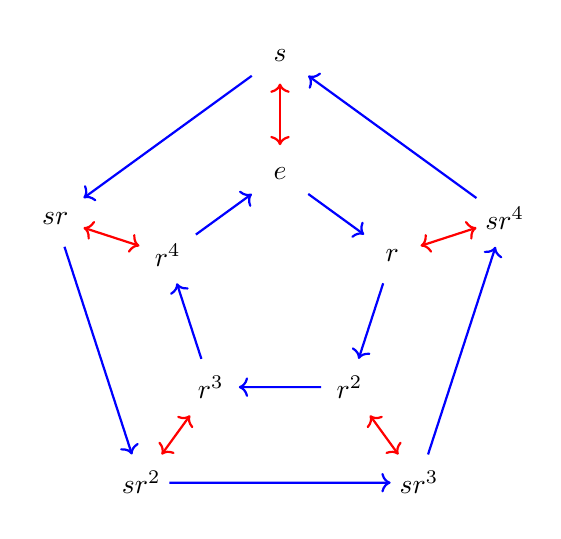
\begin{tikzpicture}[rotate=90,scale=1.5]
        \tikzstyle{vertex}=[minimum size=20pt,inner sep=0pt]

        \draw (-0*360/5:2) node[vertex] (v1) {$s$};
        \draw (-0*360/5:1) node[vertex] (v2) {$e$};
        \draw (-1*360/5:2) node[vertex] (v3) {$sr^4$};
        \draw (-1*360/5:1) node[vertex] (v4) {$r$};
        \draw (-2*360/5:2) node[vertex] (v5) {$sr^3$};
        \draw (-2*360/5:1) node[vertex] (v6) {$r^2$};
        \draw (-3*360/5:2) node[vertex] (v7) {$sr^2$};
        \draw (-3*360/5:1) node[vertex] (v8) {$r^3$};
        \draw (-4*360/5:2) node[vertex] (v9) {$sr$};
        \draw (-4*360/5:1) node[vertex] (v10) {$r^4$};

        \draw[<->, red, thick] (v2) -- (v1);
        \draw[<->, red, thick] (v4) -- (v3);
        \draw[<->, red, thick] (v6) -- (v5);
        \draw[<->, red, thick] (v8) -- (v7);
        \draw[<->, red, thick] (v10) -- (v9);

        \draw[->, blue, thick] (v2) -- (v4);
        \draw[->, blue, thick] (v4) -- (v6);
        \draw[->, blue, thick] (v6) -- (v8);
        \draw[->, blue, thick] (v8) -- (v10);
        \draw[->, blue, thick] (v10) -- (v2);

        \draw[<-, blue, thick] (v9) -- (v1);
        \draw[<-, blue, thick] (v1) -- (v3);
        \draw[<-, blue, thick] (v3) -- (v5);
        \draw[<-, blue, thick] (v5) -- (v7);
        \draw[<-, blue, thick] (v7) -- (v9);
    \end{tikzpicture}
\end{center}
where the blue arrows represent $r$ and the red arrows represent $s$.

\pagebreak
\begin{problem}
Consider the matrices
$A=\begin{pmatrix} 1&1&0 \\ 0&1&0\\ 0&0&1\end{pmatrix}$, 
$B=\begin{pmatrix} 1&0&1 \\ 0&1&0\\ 0&0&1\end{pmatrix}$,
$C=\begin{pmatrix} 1&0&0 \\ 0&1&1\\ 0&0&1\end{pmatrix}\in GL_3(\Z).$   
    \begin{enumerate}[(a)]
       \item Show that $A,B,C$ generate the Heisenberg group $H :=  \left\{ 
\begin{pmatrix}
1 & a & b \\
0 & 1 & c \\
0 & 0 & 1
\end{pmatrix}
\mid a, b, c \in \Z \right\},
$
and give a set of words in the generators $A,B,C$ (and their inverses) among which every element
of $H$ appears exactly once. 
        \item Give a presentation of $H$ in terms of the generators $A,B,C$.
Show that your relations describe $H$, rather than a larger group of
which $H$ is a quotient, by checking that any word in $A,B,C$ (and their 
inverses) reduces to one of the words you gave in part (a).
        \item Show that $H$ has polynomial growth rate, i.e.\ that the number of 
elements described by arbitrary words of length at most $N$ in $A,B,C$
and their inverses is bounded between two polynomials in $N$.
        \item The number of elements of $H$ described by words of length at most $N$
can in fact be bounded
between two polynomials of the {\em same degree} $d$ (with positive leading
coefficients). What is the value of $d$?
        \item How does your answer to the previous question change if we choose a 
different (finite) set of generators of $H$?
    \end{enumerate}
\end{problem}

\textbf{(a)} A simple matrix calculation shows that for integers $a,b,c\in \Z$ we have
\[
    C^c B^b A^a = \begin{pmatrix}
        1 & a & b\\ 0 & 1 & c \\ 0 & 0 & 1
    \end{pmatrix}
.\] 

\textbf{(b)} To describe the relations among the $A,B,C$. It suffices to calculate commutators,
\[
    [A,B]=1, \quad [B,C]=1, \quad [A,C]=B
.\] 
This is because given any word in $A,B,C$ we can use commutators to swap around any elements to arrive at some canonical form.

\textbf{(c-d)} We claim that the degree is $4$.

\begin{lemma}
    Letting $\ell$ be the length function. Then
    \[
        \ell(C^cA^aB^b)\leq \ell(c)+\ell(a)+k\sqrt{\ell(b)}
    \]
    for some constant $k$.
\end{lemma}
\begin{proof}
    By a long and tedious inductive calculation which we will not bore the graders with, we can arrive at the following commutator relationship
    \[
        [A^n, C^m] = B^{nm}
    .\]
    So $\ell(B^{nm})=2n+2m$ and the result follows.
\end{proof}

The degree $4$ part comes because the ``inverse'' of $\sqrt{\ell(b)}$ is $\ell(b)^2$ and since the other two terms are linear, so we have $1+1+2=4$.

\textbf{(e)} By the same argument as in class, it follows that for any other generating set, we can rewrite the first generating set in terms of the first generating set, and this doesn't change the asymptotics.

\pagebreak
\begin{problem}
Let $G=\langle x,y\,|\,x^2=y^3=(xy)^3=1\rangle$.
\begin{enumerate}[(a)]
    \item Show that every element of $G$ can be expressed as $y^k$ or $y^kxy^\ell$ for some $k,\ell\in \Z/3$.
    \item Construct a homomorphism from $G$ to the alternating group $A_4$, and use it to show that $G\simeq A_4$.
\end{enumerate}
\end{problem}

\textbf{(a)} Every element in $G$ can clearly be expressed as some sequence of $x$'s and $y^\ell$'s for some $\ell \in \{1,2\}$. To prove that such a word can be reduced to something of the form $y^kxy^\ell$, we can use induction on the number on $x$'s in the expression. Before doing this, we can derive some simple relations for this group. Note that 
\[
    \begin{aligned}
        (xy)^3=xyxyxy&=1\\
        xyxy&=y^2x\\
        xyx&=y^2xy^2.
    \end{aligned}
\]
Similarly we can derive $xy^2x=yxy$. So for any word in $x,y,y^2$, whenever we have more than one $x$ term we can use the relations to reduce it to a single $x$ term. Doing this repeatedly gives us an expression with less than one $x$ term, so either $y^k$ or $y^kxy^\ell$.

\textbf{(b)} Consider the homomorphism $G\to A_4$ given by $x\mapsto (12)(34)$ and $y\mapsto (123)$. Then $x^2=1$, $y^3=1$, and $xy=(134)$ so $(xy)^3=1$. So this map is a homorphism. To prove isomorphism, it suffices to check that all $12$ expressions from (a) all map to distinct elements in $A_4$. This is a straightforward computation. So $G\cong A_4$.

\pagebreak
\begin{problem}[optional, extra credit] Consider the group $SL_2(\F_3)$ of $2\times 2$
matrices with entries in $\F_3$ and determinant 1, and its quotient
$PSL_2(\F_3)=SL_2(\F_3)/\{\pm I\}$ by the normal subgroup $\{\pm I\}$.
There is a natural homomorphism $\varphi$ from $PSL_2(\Z)=SL_2(\Z)/\{\pm I\}$ to
$PSL_2(\F_3)$ given by reducing coefficients mod 3. The kernel of $\varphi$
is called the {\em congruence subgroup} $\Gamma(3)\subset PSL_2(\Z)$.

Show that the congruence subgroup $\Gamma(3)$ is normally generated by 
$$M=\begin{pmatrix}1&3\\0&1\end{pmatrix},$$ i.e.\ that it is the smallest
normal subgroup of $PSL_2(\Z)$ which contains $M$.
\end{problem}

\textit{(Hint: Recall from lecture that $PSL_2(\Z)$ has a presentation with
generators 
$S=\left(\begin{smallmatrix}0&-1\\1&\ \,\,0\end{smallmatrix}\right)$ and
$R=\left(\begin{smallmatrix}0&-1\\1&\ \,\,1\end{smallmatrix}\right)$
and relations $S^2=R^3=1$.
First show that $PSL_2(\F_3)\simeq A_4$, e.g.\ by considering the
action on subspaces of $(\F_3)^2$ as in HW8 and HW9; then
use the result of Problem 7).}

We've proven on an earlier problem set that $PGL_2(\F_3)\cong S_4$, and since $S_4$ has a unique index $2$ subgroup it follows that $PSL_2(\F_3)\cong A_4$. So by Problem~7 $PSL_2(\F_3)$ has presentation
\[
    PSL_2(\F_3) = \big\langle S, R \mid S^2=R^3=1, (SR)^3=1 \big\rangle
.\] 
Using the hint, let $S,R$ be as above. Then
\[
    PSL_2(\Z) =\big\langle S, R \mid S^2=R^3=1 \big\rangle
.\] 

Then the kernel of the map $\varphi : PSL_2(\Z) \to PSL_2(\F_3)$ is exactly the normal subgroup $\big\langle (SR)^3 \big\rangle$. Since 
\[
    (SR)^3 = \begin{pmatrix}
        1&3\\ 0&1
    \end{pmatrix}
,\]
we are done.

\end{document}
